\section{任务二}
根据任务一找到的新4轮高概率差分，要寻找所有对应的差分路线，思路为遍历所有$2^{16}$种输入差分对，即$x in \{0,1,\dots2^{16} - 1\}$、$x' = x\oplus \delta_{in}$，
记录下4轮加密过程中每一轮的中间异或结果，当满足输出差分$y \oplus y' = \delta_{out}$时，该路线即为所要求的4轮差分的差分路线，将该路线记录下来，最后输出所有差分路线并计算概率(注意这里按照输入是有序对时共$2^16$种满足条件的差分对，若按照无序对考察，则差分路线和总的差分对数量均减半，但最终概率不变)，计算概率为:
$$
P = \frac{\#{x:F^4(x) \oplus F^4(x \oplus \delta_{in}) = \delta_{out}}}{2^{16}}
$$
按照上述思路编写代码，运行结果如下:
\begin{figure}[H]
    \centering
    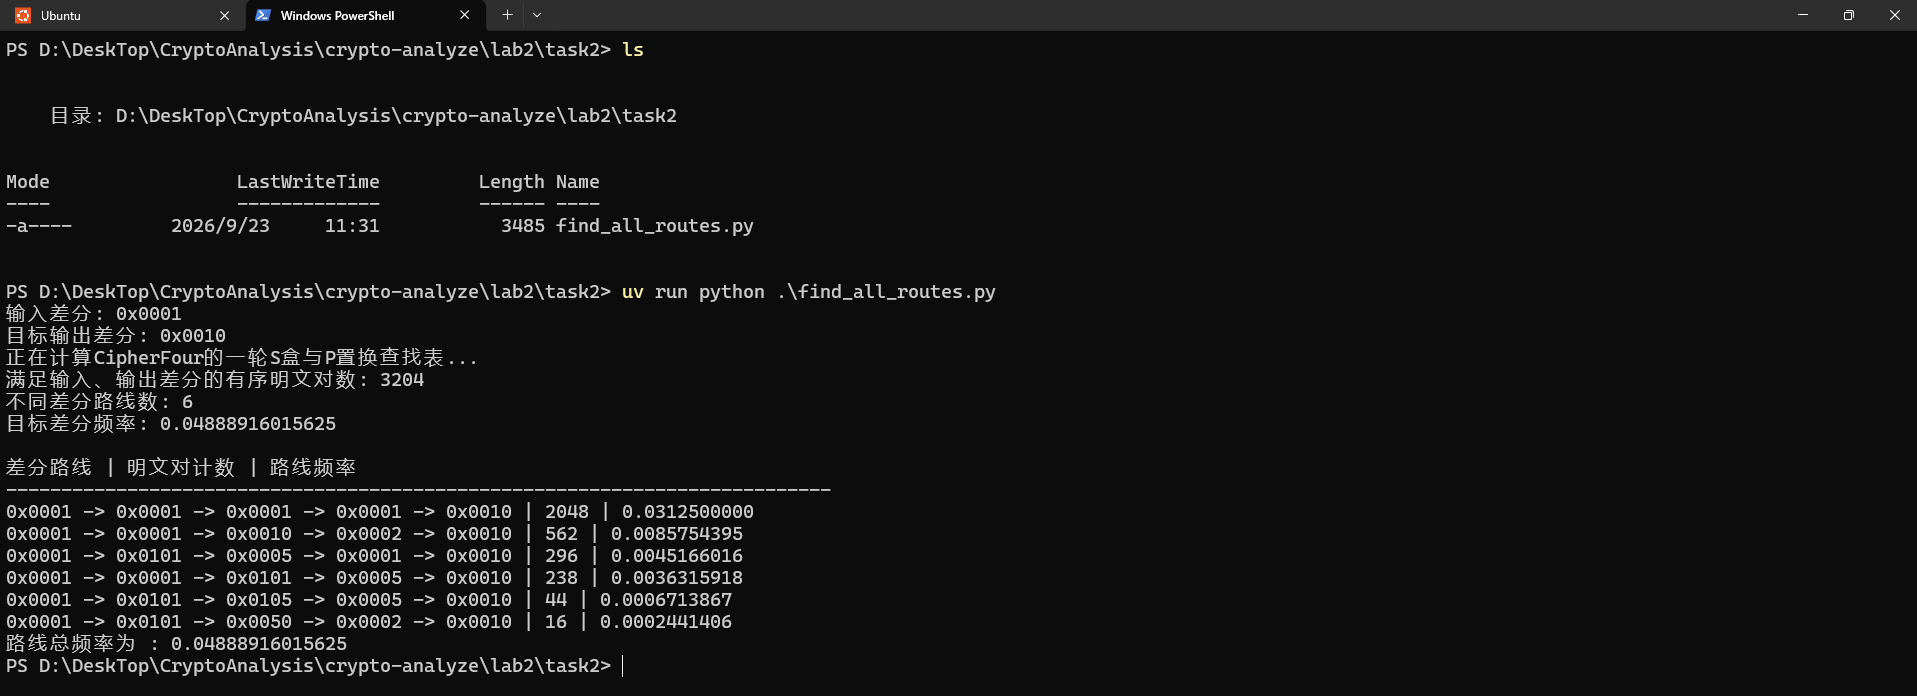
\includegraphics[width = 1\textwidth]{figures/task2_routes.png}
    \caption{所有新4轮差分路线}
\end{figure}
